\section{Slice nesting at the cylinder--slab transition}
\label{nest:section}

We consider the three-vertex pattern at volume $V=1/\pi$, under the
contradictory assumption $A\leq1$.  The slicing direction is the missing
axis, so that the top slices are empty.  Proposition
\ref{slice:three-second-parameters} gives
$0.64\leq h\leq2.25$ and $s\geq t=t(h)$, where
\eqref{slice:t-definition} defines $t$ by
$h^2t^2=\pi(1-t)$.  In particular, $h>0$ and $0<t<1$.
We use the flux identity
\[
 \int_{\partial E_z}\alpha\,d\ell=hv(z),\qquad p(0)=hs,
\]
from \eqref{slice:three-flux}, and the coarea identities
\eqref{slice:coarea}.  All perimeters in this Section are relative to the
unit square.  All terminating decimals denote exact rational numbers.

The argument first gives a lower bound depending only on $h$ and $s$.
It then improves that bound on an interval of slice areas by retaining
the fact that every slice is contained in the bottom slice.  This is
especially useful when a slice changes from a strip to the complement
of a corner region.

\subsection{An integrated flux inequality}

Fix $\lambda=0.98$. Subtracting $\lambda$ times the flux from the
surface-area coarea density gives $1/\alpha-\lambda\alpha$, whereas the
decrease of slice area has density $\sqrt{1-\alpha^2}/\alpha$.
At a constant value $0<\alpha<1$, their ratio is $g(\alpha)$, where
\[
 g(X)=\frac{1-\lambda X^2}{\sqrt{1-X^2}},\qquad 0\leq X<1.
\]
The flux determines only the arclength mean $hv/p$ of $\alpha$,
not its pointwise values. The next lemma uses convexity to obtain
a whole-slice comparison from this mean. To make that comparison
compatible with perimeter lower bounds, we use a non-increasing
minorant of $g$: replacing $p$ by a smaller quantity increases
the argument $hv/p$ and does not increase the resulting lower bound.

Set
\begin{equation}\label{nest:weight}
 \begin{gathered}
 D=\frac{\sqrt{48}}7,\qquad \ell=0.28,\\
 G(X)=g(X_0),\qquad X_0=\min\{X,D\},\quad X\geq0.
 \end{gathered}
\end{equation}
Direct differentiation gives
\begin{equation}\label{nest:weight-derivative}
 -\frac{d}{dr}g(\sqrt r)
   =\frac{0.48-0.49r}{(1-r)^{3/2}},\qquad 0\leq r<1.
\end{equation}
Thus $g$ decreases up to $D$, increases thereafter, and
$g(D)=7/25=\ell$.  Consequently $G$ is non-increasing, takes values
in $[\ell,1]$, and satisfies $G(X)\leq g(X)$ for $0\leq X<1$.
Its definition for $X\geq1$ also covers perimeter lower bounds
for which the substituted argument exceeds one.

\begin{lemma}[Integrated flux]\label{nest:integrated-flux}
At every nonempty regular slice, with area $v$ and perimeter $p$,
\begin{equation}\label{nest:jensen}
 \int_{\partial E_z}\frac{d\ell}{\alpha}-\lambda hv
 \geq
 G(hv/p)\int_{\partial E_z}
       \frac{\sqrt{1-\alpha^2}}{\alpha}\,d\ell.
\end{equation}
If a nonnegative measurable function $\gamma$ satisfies
$G(hv(z)/p(z))\geq\gamma(v(z))$ at the nonempty regular levels, then
\begin{equation}\label{nest:area-coordinate}
 A\geq\frac{\lambda h}{\pi}+\int_0^s\gamma(v)\,dv.
\end{equation}
\end{lemma}

\begin{proof}
For fixed $J\in[0,1]$, let
\[
 f_J(X)=\frac1X-\lambda X-J\frac{\sqrt{1-X^2}}X,
 \qquad 0<X\leq1.
\]
On $(0,1)$,
\[
 X^3f_J''(X)=2-J\frac{2-3X^2}{(1-X^2)^{3/2}}\geq0.
\]
Indeed, the function $(2-3r)/(1-r)^{3/2}$ decreases from $2$ to $0$
on $[0,2/3]$, its derivative being
$-3r/[2(1-r)^{5/2}]$; it is nonpositive on $[2/3,1)$.
Convexity extends to the continuous endpoint value at $X=1$.

Use normalized arclength on the slice curve as a probability measure.
The flux identity says that the mean of $\alpha$ is
$m=hv/p\in(0,1]$.  Take $J=G(m)$.  For $m<1$,
\[
 f_J(m)=\frac{\sqrt{1-m^2}}m\bigl(g(m)-G(m)\bigr)\geq0;
\]
for $m=1$, $f_J(1)=1-\lambda>0$.  Jensen's inequality now yields
$\int f_J(\alpha)\,d\ell\geq0$, which is
\eqref{nest:jensen}.

Down-set position gives $N_z\geq0$, hence
$\sqrt{1-\alpha^2}=N_z$.  The coarea identities therefore turn
\eqref{nest:jensen} into
\[
 A-\lambda hV
 \geq\int_0^1G(hv(z)/p(z))\,(-v'(z))\,dz
 \geq\int_0^1\gamma(v(z))\,(-v'(z))\,dz.
\]
The integrands are set to zero at empty or exceptional levels.
Lemma~\ref{slice:regularity}, with $r=0$, identifies the last integral
with $\int_0^s\gamma(v)\,dv$. Since $V=1/\pi$, this proves
\eqref{nest:area-coordinate}.
\end{proof}

\begin{lemma}[Planar patterns and the baseline bound]
\label{nest:planar-patterns}
Every nonempty regular slice satisfies
\begin{equation}\label{nest:planar-bound}
 p\geq p_*(v):=
 \min\{\sqrt{\pi v},\ 1,\ \sqrt{\pi(1-v)}\}.
\end{equation}
Put $a_0=1/\pi$, $b_0=1-1/\pi$, and define
\begin{equation}\label{nest:baseline}
 B(h)=\frac{\lambda h}{\pi}
       +\int_0^{t(h)}G\!\left(\frac{hv}{p_*(v)}\right)\,dv-1.
\end{equation}
At $v=0$ the argument in the integrand is understood by its limit.
Then
\begin{equation}\label{nest:baseline-slack}
 A-1\geq B(h)+\ell(s-t).
\end{equation}
\end{lemma}

\begin{proof}
The far vertex $(1,1)$ is absent even from the bottom slice and hence
from every slice.  A nonempty regular slice has, by monotonicity,
one, two adjacent, or three occupied square vertices.  In the first
case the slice is confined to the occupied corner.  Reflection across
its two adjacent sides gives a bounded planar set of area $4v$ and
perimeter $4p$; the Euclidean isoperimetric inequality gives
$p^2\geq\pi v$.  In the three-vertex case the same argument applies
to the opposite-corner complement and gives $p^2\geq\pi(1-v)$.

In the two-vertex case, after interchanging the square coordinates if
necessary, the occupied vertices form the bottom edge.  This entire
edge is occupied and the opposite edge is vacant.  Each vertical
segment crosses the separating curve exactly once: monotonicity
gives uniqueness, and the strict normal inequality gives a transverse
crossing.  The implicit function theorem, also in the reflected
endpoint neighborhoods, writes the curve as a single decreasing
graph $y=f(x)$ for $0\leq x\leq1$.  Its length is at least $1$.
These arguments establish \eqref{nest:planar-bound}, including both
strip orientations.

Since $G$ is non-increasing, \eqref{nest:planar-bound} implies
$G(hv/p)\geq G(hv/p_*(v))$.  Apply
Lemma~\ref{nest:integrated-flux} and use $s\geq t$ and $G\geq\ell$
on the remaining interval $[t,s]$ to obtain
\eqref{nest:baseline-slack}.
\end{proof}

The scalar estimates in Appendix~\ref{num:section} show that $B(h)$
suffices outside $[1.02,1.62]$ but is negative at $h=1.46$.
The slack $s-t$ contributes $\ell(s-t)$ directly. When this slack is
small, the bottom complement constrains both edge extents; nesting
then bounds each strip's smaller endpoint and forces a length excess.
We quantify these two gains and minimize their sum over the slack.

\subsection{The bottom slice controls both strip orientations}

In the remainder of the geometric improvement assume
$1.02\leq h\leq1.62$.  Let $L_x,L_y$ be the extents of the bottom
complement along the sides $y=1,x=1$, respectively.  They are measured
from its corner $(1,1)$ and need not be equal.
Figure~\ref{nest:containment-figure} shows how each extent constrains
the endpoint of a contained strip in the corresponding orientation.

\begin{figure}[ht]
\centering
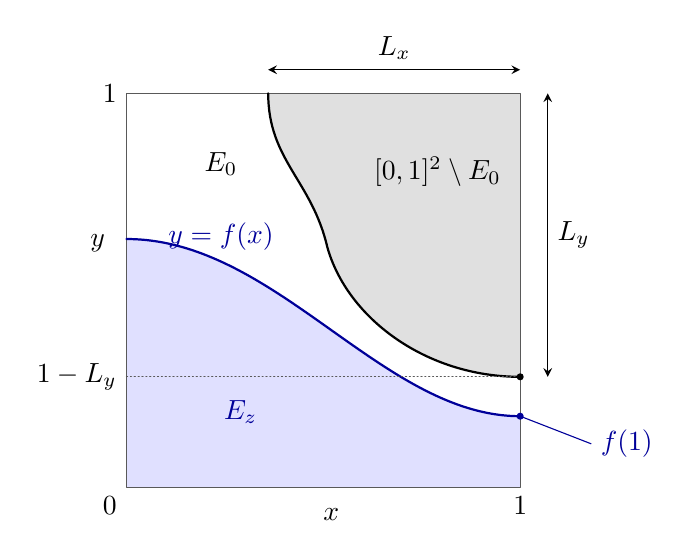
\begin{tikzpicture}[x=5cm,y=5cm,>=stealth,line cap=round,line join=round]
 \fill[black!12] (0.36,1) -- (1,1) -- (1,0.28)
   .. controls (0.76,0.28) and (0.56,0.43) .. (0.51,0.61)
   .. controls (0.47,0.78) and (0.36,0.83) .. (0.36,1) -- cycle;
 \fill[blue!12] (0,0) -- (1,0) -- (1,0.18)
   .. controls (0.65,0.18) and (0.38,0.63) .. (0,0.63) -- cycle;
 \draw[black!65] (0,0) rectangle (1,1);
 \draw[thick] (0.36,1)
   .. controls (0.36,0.83) and (0.47,0.78) .. (0.51,0.61)
   .. controls (0.56,0.43) and (0.76,0.28) .. (1,0.28);
 \draw[thick,blue!60!black] (0,0.63)
   .. controls (0.38,0.63) and (0.65,0.18) .. (1,0.18);
 \draw[<->] (0.36,1.06) -- node[above] {$L_x$} (1,1.06);
 \draw[<->] (1.07,0.28) -- node[right] {$L_y$} (1.07,1);
 \draw[densely dotted,black!65] (0,0.28) -- (1,0.28);
 \node[left] at (0,0.28) {$1-L_y$};
 \fill (1,0.28) circle[radius=0.009];
 \fill[blue!60!black] (1,0.18) circle[radius=0.009];
 \draw[blue!60!black] (1,0.18) -- (1.18,0.11);
 \node[right,blue!60!black] at (1.18,0.11) {$f(1)$};
 \node at (0.79,0.80) {$[0,1]^2\setminus E_0$};
 \node[blue!60!black] at (0.29,0.19) {$E_z$};
 \node at (0.24,0.82) {$E_0$};
 \node[blue!60!black,above] at (0.24,0.575) {$y=f(x)$};
 \node[below left] at (0,0) {$0$};
 \node[below] at (1,0) {$1$};
 \node[left] at (0,1) {$1$};
 \node[below] at (0.52,-0.03) {$x$};
 \node[left] at (-0.03,0.62) {$y$};
\end{tikzpicture}
\caption{Nesting constrains a strip through the bottom complement.
The shaded strip $E_z=\{(x,y):0\leq y\leq f(x)\}$ lies in $E_0$,
so its smaller endpoint satisfies $f(1)\leq1-L_y$.
Interchanging $x$ and $y$ gives the bound using $L_x$ for the other
strip orientation. The curves and the unequal extents are schematic;
no convexity or circular shape is assumed.}
\label{nest:containment-figure}
\end{figure}


\begin{lemma}[Bottom calibration and nesting]
\label{nest:bottom-calibration}
Each $L\in\{L_x,L_y\}$ satisfies
\begin{equation}\label{nest:extent-bound}
 hs\geq\frac{1-s}{L}+\frac{\pi L}{4}.
\end{equation}
Consequently, a strip slice, written as a decreasing subgraph across
either square coordinate, has smaller endpoint at most
\begin{equation}\label{nest:endpoint-bound}
 \begin{split}
 e&=1-\frac2\pi
       \left(hs-\sqrt{h^2s^2-\pi(1-s)}\right)\\
  &\leq1-\frac{2ht}{\pi}+QY,
 \qquad
 Y=\sqrt{s-t},\qquad
 Q=\frac2\pi\sqrt{\pi+2h^2t}.
 \end{split}
\end{equation}
\end{lemma}

\begin{proof}
Use coordinates $(\xi,\eta)$ measured from the complement's corner,
so that its monotone separating curve runs from $(0,L_y)$ to
$(L_x,0)$ with $d\xi\geq0$, $d\eta\leq0$.
For $L=L_y$, the vector
\[
 \left(\frac\eta L,-\sqrt{1-\frac{\eta^2}{L^2}}\right)
\]
has unit length.  Pairing it with the tangent differential and
integrating gives
\[
 \begin{split}
 hs&\geq
 \frac1L\int\eta\,d\xi
   -\int\sqrt{1-\eta^2/L^2}\,d\eta\\
 &=\frac{1-s}{L}+\int_0^L\sqrt{1-\eta^2/L^2}\,d\eta
 =\frac{1-s}{L}+\frac{\pi L}4.
 \end{split}
\]
The first integral is the complement area.  This calculation uses
only monotonicity of the curve, and so requires no convexity.
Exchanging $\xi$ and $\eta$ proves the same estimate for $L_x$.
Both extents are positive, because the complement has positive area.

Solving the quadratic inequality \eqref{nest:extent-bound} gives,
for each extent,
\[
 L\geq\frac2\pi
    \left(hs-\sqrt{h^2s^2-\pi(1-s)}\right).
\]
The discriminant is nonnegative by $hs\geq\sqrt{\pi(1-s)}$.
A strip $y=f(x)$ is contained in the bottom slice, so its smaller
endpoint satisfies $f(1)\leq1-L_y\leq e$.  For a strip $x=f(y)$
the same argument uses $L_x$.  Thus one common bound controls both
orientations without imposing a symmetry on the two extents.

Finally, write $s=t+Y^2$ and use $h^2t^2=\pi(1-t)$ to obtain
\[
 h^2s^2-\pi(1-s)
   =(\pi+2h^2t)Y^2+h^2Y^4.
\]
Its square root is at most
$\sqrt{\pi+2h^2t}\,Y+hY^2$.  Substituting this upper bound in
$e$ cancels the term $hY^2$ coming from $hs$, and proves
\eqref{nest:endpoint-bound}.
\end{proof}

We seek this excess on an interval $[u-\delta,u]$ within the middle
branch of $p_*$; the choice of $u$ also keeps $hv\leq0.96<D$.
With $Q,Y$ as in \eqref{nest:endpoint-bound}, set
\begin{equation}\label{nest:gain-parameters}
 \begin{gathered}
 u=\min\{b_0,0.96/h\},\qquad
 P=u-1+\frac{2ht}{\pi},\\
 d_m=0.21,\qquad c=2.7,\qquad
 \delta=\min\{d_m,(P-QY)_+\},
 \end{gathered}
\end{equation}
where $x_+=\max\{x,0\}$.
Here $P-QY$ is a lower bound for the gap between $u$ and the smaller
strip endpoint, and $\delta$ is its positive part capped at $d_m$.

\begin{lemma}[Placement and the three slice types]
\label{nest:shape-gain}
On $1.02\leq h\leq1.62$ one has
\begin{equation}\label{nest:interval-placement}
 u-d_m\geq\frac{1033}{2700}>0.38>a_0,
 \qquad u\leq b_0,\qquad u<t\leq s,\qquad hu\leq0.96.
\end{equation}
Define
\begin{equation}\label{nest:shape-function}
 H(q)=\min\left\{q^2,\frac{\pi(1-q)}{c d_m}\right\},
 \qquad 0\leq q\leq1.
\end{equation}
If $\delta>0$, put $q=(v-u+\delta)/\delta$ for
$u-\delta\leq v\leq u$. Every regular slice in this area interval satisfies
\begin{equation}\label{nest:improved-perimeter}
 p^2\geq1+c\delta^2H(q).
\end{equation}
\end{lemma}

\begin{proof}
The definition of $u$ gives $u\geq0.96/1.62=16/27$,
$u\leq b_0$, and $hu\leq0.96$.  Hence the first assertion follows
from $16/27-0.21=1033/2700$, using $\pi>3$.
Moreover,
\[
 h^2u^2\leq0.96^2<1\leq\pi(1-u).
\]
The function $x\mapsto h^2x^2+\pi x-\pi$ is strictly increasing
for $x\geq0$ and vanishes at $t$, so $u<t$.
This proves \eqref{nest:interval-placement}; in particular
$[u-\delta,u]\subset[a_0,b_0]\cap[0,s]$, where $p_*=1$.
For the remaining assertion assume $\delta>0$. The definition of
$\delta$ and \eqref{nest:endpoint-bound} then give
\begin{equation}\label{nest:strip-endpoint}
 e\leq u-P+QY\leq u-\delta.
\end{equation}

We verify \eqref{nest:improved-perimeter} separately for all three
slice types of Lemma~\ref{nest:planar-patterns}.

\emph{Occupied corner.}
Here $p^2\geq\pi v$.  Since $v>0.38$ and $\pi>3$,
\[
 p^2-1>0.14>c d_m^2=0.11907\geq c\delta^2H(q).
\]
In the last step we used $H(q)\leq q^2\leq1$.

\emph{Opposite-corner complement.}
Here $p^2\geq\pi(1-v)$, and $v=u-\delta+\delta q$ gives
\[
 \begin{split}
 p^2-1&\geq\pi(b_0-v)
 \geq\pi\delta(1-q)\\
 &\geq c\delta^2\frac{\pi(1-q)}{c d_m}
 \geq c\delta^2H(q).
 \end{split}
\]
This includes the endpoint $q=1$, $u=b_0$, where $H(1)=0$.

\emph{Strip.}
Write the strip as $y=f(x)$, interchanging the two square coordinates
if required.  Its smooth decreasing graph has $f(1)\leq e$ by
Lemma~\ref{nest:bottom-calibration}.  Integration by parts and
\eqref{nest:strip-endpoint} give
\[
 \int_0^1x|df|=\int_0^1f(x)\,dx-f(1)
    =v-f(1)\geq v-u+\delta=:j=\delta q.
\]
Set $k=2.5j\leq2.5d_m=0.525$.  Pair the graph tangent
$(dx,|df|)$ with the unit vector
$(\sqrt{1-k^2x^2},kx)$ to obtain
\begin{equation}\label{nest:strip-calibration}
 p\geq kj+\int_0^1\sqrt{1-k^2x^2}\,dx.
\end{equation}
For $0\leq w\leq0.525^2$,
\[
 \sqrt{1-w}\geq1-\frac w2-\frac{w^2}5.
\]
Indeed the right side is positive and its square minus $1-w$ is
$w^2(-3/20+w/5+w^2/25)\leq0$; the expression in parentheses is
increasing and is negative at $w=0.525^2$.
It follows from \eqref{nest:strip-calibration} that
\[
 \begin{split}
 p&\geq1+\left(\frac{35}{24}-\frac{25j^2}{16}\right)j^2\\
  &\geq1+\frac{26677}{19200}j^2
   \geq1+1.35j^2.
 \end{split}
\]
Squaring gives $p^2\geq1+2.7j^2\geq1+c\delta^2H(q)$.
This establishes the same estimate for every slice type, even if
the type or strip orientation changes within the area interval.
Exceptional levels are not needed in this argument and have zero
measure after the substitution in Lemma~\ref{nest:integrated-flux}.
\end{proof}

\subsection{From perimeter improvement to an area gain}

The perimeter improvement has size proportional to $\delta^2$ on
an interval of slice areas of width $\delta$. We will show that it
adds an explicit positive multiple of $\delta^3$ to the total area
bound. The derivative estimate below converts the improvement of $p$
into an improvement of $G(hv/p)$; the moments of $H$ then average
that improvement over the interval. Together with the already obtained
term $\ell(s-t)$, this will leave a one-variable minimization over
the unknown bottom area $s$.

\begin{lemma}[Derivative estimate]\label{nest:derivative-bound}
For $0\leq X\leq0.96$,
\begin{equation}\label{nest:derivative-inequality}
 \frac{0.48-0.49X^2}{(1-X^2)^{3/2}}\geq0.91X.
\end{equation}
\end{lemma}

\begin{proof}
The assertion is immediate at $X=0$.  For $X>0$, divide the left
side by $X$ and write the result as
\[
 \frac{N(X)}{D_1(X)},\qquad
 N(X)=0.49-\frac{0.01}{1-X^2},\qquad
 D_1(X)=X\sqrt{1-X^2}.
\]
The numerator decreases; the denominator is at most $1/2$ everywhere
and decreases for $X\geq1/\sqrt2$.  The following rational bounds
therefore suffice:
\[
\begin{array}{c|cc}
 \text{interval for }X&N(X)\text{ lower bound}&D_1(X)\text{ upper bound}\\
 \hline
 {[0,0.84]}&0.456&0.50\\
 {[0.84,0.89]}&0.44&0.46\\
 {[0.89,0.94]}&0.40&0.41\\
 {[0.94,0.96]}&0.36&0.33
\end{array}
\]
For clarity, each entry is certified by arithmetic on rational
numbers.  If $b$ is the right endpoint and $n$ the numerator bound,
the four values of $(0.49-n)(1-b^2)-0.01$ are respectively
$0.0000096$, $0.000395$, $0.000476$, $0.000192$, all positive.
For the last three rows the values of $D_1(a)^2$ at the left
endpoints are $0.20772864$, $0.16467759$, $0.10285104$, smaller
than $0.46^2$, $0.41^2$, $0.33^2$ respectively.
Finally each numerator lower bound exceeds $0.91$ times the
denominator upper bound; the respective differences are
$0.001$, $0.0214$, $0.0269$, $0.0597$.
\end{proof}

Define the moments and a perimeter bound associated with $H$ by
\begin{equation}\label{nest:shape-moments}
 M=\int_0^1H(q)\,dq,\qquad
 q_m=\frac{\int_0^1qH(q)\,dq}{M},\qquad
 p_2=1+c d_m^2\max_{[0,1]}H.
\end{equation}

\begin{lemma}[Uniform coefficient]\label{nest:coefficient-bound}
The constants in \eqref{nest:shape-moments} satisfy
\begin{equation}\label{nest:moment-bounds}
 M>0.2659,\qquad q_m>0.697,\qquad p_2<1.09.
\end{equation}
For $1.02\leq h\leq1.62$,
\begin{equation}\label{nest:coefficient-inequality}
 \frac{0.91cM}{p_2^{3/2}}
       \bigl[h(u-(1-q_m)d_m)\bigr]^3
 \geq C_0(h),
\end{equation}
where
\begin{equation}\label{nest:gain-coefficient}
 C_0(h)=\min\{0.134h^3,0.36\}.
\end{equation}
\end{lemma}

\begin{proof}
The two branches of $H$ meet once, at
\[
 \theta=\frac{2}{1+\sqrt{1+4cd_m/\pi}},
 \qquad cd_m\theta^2=\pi(1-\theta).
\]
Thus $H(q)=q^2$ up to $\theta$ and
$H(q)=\pi(1-q)/(cd_m)$ thereafter, with maximum $\theta^2$.
Integration, followed by the identity
$\pi/(cd_m)=\theta^2/(1-\theta)$, gives
\begin{equation}\label{nest:exact-moments}
 \begin{split}
 M&=\frac{\theta^3}3+
       \frac{\pi(1-\theta)^2}{2cd_m}
     =\frac{\theta^2(3-\theta)}6,\\
 \int_0^1qH(q)\,dq
   &=\frac{\theta^4}4+
       \frac{\pi(1-\theta)^2(1+2\theta)}{6cd_m},\\
 q_m&=\frac{2+2\theta-\theta^2}{2(3-\theta)},\qquad
 p_2=1+cd_m^2\theta^2.
 \end{split}
\end{equation}
Only $3.14<\pi<22/7$ is needed to bound these expressions.
The function $0.567x^2-\pi(1-x)$ increases on $[0,1]$, and
\[
 \begin{split}
 0.567(32/37)^2-3.14(5/37)&=-\frac{73}{342250}<0,\\
 0.567(13/15)^2-(22/7)(2/15)&=\frac{3587}{525000}>0.
 \end{split}
\]
It follows that $32/37<\theta<13/15$.
Both $\theta^2(3-\theta)/6$ and
$(2+2\theta-\theta^2)/(2(3-\theta))$ increase on $(0,1)$;
for the latter, the derivative is
$(\theta-2)(\theta-4)/(2(3-\theta)^2)>0$.
Consequently
\[
 M>\frac{40448}{151959}>0.2659,
 \qquad q_m>\frac{2041}{2923}>0.697,
 \qquad p_2<\frac{2723587}{2500000}<1.09.
\]
This proves \eqref{nest:moment-bounds}.

Here are explicit rational margins for the remaining coefficient.
Put $\beta_0=0.303d_m=0.06363$.  The bounds just proved imply
\[
 \frac{0.91cM}{p_2^{3/2}}
   >\frac{0.91\cdot2.7\cdot0.2659}{1.09^{3/2}}>0.574.
\]
The last inequality follows by squaring positive quantities, since
\[
 (0.91\cdot2.7\cdot0.2659)^2
      -0.574^2\,1.09^3
      =\frac{14121304169}{10^{14}}>0.
\]
Also $(1-q_m)d_m<\beta_0$.
If $u=b_0$, then
$u-\beta_0>1-1/3.14-0.06363>0.617$, and
\[
 0.574(0.617)^3=0.134824054862>0.134.
\]
Hence the left side of \eqref{nest:coefficient-inequality} exceeds
$0.134h^3$.  If $u=0.96/h$, then
\[
 h(u-\beta_0)\geq0.96-1.62\beta_0
     =0.8569194>0.856,
 \qquad
 0.574(0.856)^3=0.360025437184>0.36.
\]
Both branches therefore dominate $C_0(h)$, including their common
endpoint and the switch in the definition of $C_0$.
\end{proof}

\begin{proposition}[The nesting area bound]\label{nest:area-bound}
For the three-vertex configuration at $V=1/\pi$ with $A\leq1$,
\[
 A-1\geq B(h)\qquad(0.64\leq h\leq2.25).
\]
On $1.02\leq h\leq1.62$ define
\begin{equation}\label{nest:gain-definition}
 S(h)=\inf_{y\geq0}
 \left\{\ell y^2+
   C_0(h)\min\{d_m,(P-Qy)_+\}^{\,3}\right\}.
\end{equation}
Then
\begin{equation}\label{nest:area-gain}
 A-1\geq B(h)+S(h).
\end{equation}
\end{proposition}

\begin{proof}
The first assertion follows from \eqref{nest:baseline-slack}.
For the second, first suppose $\delta>0$ and restrict to the area
interval $[u-\delta,u]$ of Lemma~\ref{nest:shape-gain}.  Put
$K=c\delta^2H(q)$.  Since $p\geq\sqrt{1+K}$ and $G$ is
non-increasing,
\[
 G(hv/p)\geq G\!\left(\frac{hv}{\sqrt{1+K}}\right).
\]
On this interval the baseline uses $p_*=1$, and
$hv\leq hu\leq0.96<D$.
Thus the whole squared-argument interval
$[(hv)^2/(1+K),(hv)^2]$ lies in the differentiable branch of $G$.
By \eqref{nest:weight-derivative} and
Lemma~\ref{nest:derivative-bound},
\begin{equation}\label{nest:pointwise-gain}
 \begin{split}
 G\!\left(\frac{hv}{\sqrt{1+K}}\right)-G(hv)
 &\geq \int_{(hv)^2/(1+K)}^{(hv)^2}0.91\sqrt r\,dr\\
 &\geq\frac{0.91(hv)^3K}{(1+K)^{3/2}}
 \geq\frac{0.91(hv)^3c\delta^2H(q)}{p_2^{3/2}}.
 \end{split}
\end{equation}
The second inequality bounds $\sqrt r$ below by its value at the
left endpoint, and the last uses $1+K\leq p_2$.

Changing variables $v=u-\delta+\delta q$ supplies a further factor
$\delta$.  Jensen's inequality for the convex function $v^3$ on
$v\geq0$, with probability density $H/M$, gives
\[
 \begin{split}
 \int_0^1 (u-\delta+\delta q)^3H(q)\,dq
 &\geq M\bigl(u-(1-q_m)\delta\bigr)^3\\
 &\geq M\bigl(u-(1-q_m)d_m\bigr)^3.
 \end{split}
\]
All bases are positive by \eqref{nest:interval-placement}.
Integrating \eqref{nest:pointwise-gain} and applying
Lemma~\ref{nest:coefficient-bound} therefore gives an additional
area contribution at least $C_0\delta^3$ beyond the baseline.
If $\delta=0$, that conclusion holds trivially with zero gain;
no variable $q$ is then introduced.

Together with the baseline contribution from $[t,s]$, this proves
\[
 A-1\geq B(h)+\ell(s-t)+
 C_0\min\{d_m,(P-Q\sqrt{s-t})_+\}^{\,3}.
\]
Taking the infimum over all $y\geq0$ weakens this inequality and
yields \eqref{nest:area-gain}.
\end{proof}

Lemma~\ref{nest:s-formula} in Appendix~\ref{num:section} gives an
explicit formula for the scalar infimum $S$.
